\section{Founding cohorts and early survival}
\label{m:app:cohorts}

This appendix collects the early-generation calculations for the binary
Galton--Watson process that later modelling chapters draw on: the survival
probability of a founding cohort of size $k$, the arithmetic of the first few
generations near criticality, and the conditioning effect known as the push of
the past.

\subsection*{The first generations near criticality}

Return to the binary process of \cref{m:sec:gw} near critical, either just below
or just above. With the probability of division $p$ and of death $1-p$ each close
to a half, a lineage dies at its first round almost half the time. Should it
survive one generation, both its offspring fail at their own first attempt with
probability around $0.25$, so the lineage reaches the second generation only with
probability about $0.375$:
\begin{equation*}
0.375 \approx
\underbrace{(1-0.5)}_{\text{no extinction at the first step}}\times
\underbrace{(1-0.5\times0.5)}_{\text{nor at the second}} .
\end{equation*}

More generally, survival to a given generation is obtained by iterating the \pgf{}.
With $\phi(z)=pz^2+(1-p)$ from \cref{m:eq:pgfbinary}, the extinction and survival
probabilities follow from
\begin{equation}
\label{m:eq:ext}
u_{n+1} = p\,u_n^2 + 1-p,
\qquad
S_{n+1} = 2pS_n - pS_n^2 ,
\end{equation}
started at $u_0=0$, $S_0=1$. At exactly critical branching this gives, for
$n=1,2,3,4$,
\begin{equation*}
u_n = 0.500,\ 0.625,\ 0.695,\ 0.741\qquad(3\ \text{s.f.}),
\end{equation*}
so the probability of survival decays quickly over the first few rounds of
division, and does so almost as fast just above criticality as just below.
\Cref{m:fig:earlySn} makes the point: whatever advantage supercriticality
confers, it is not an early-generation advantage.

\begin{figure}[ht]
\centering
  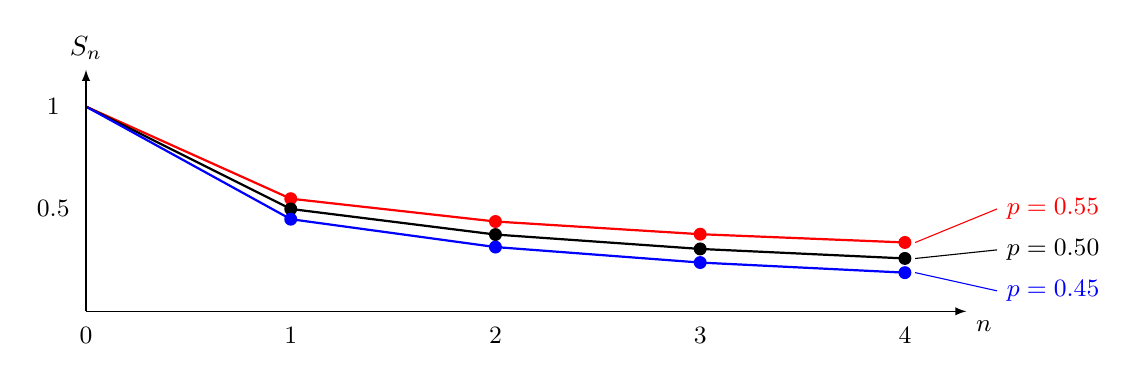
\begin{tikzpicture}[scale = 2.6]
    \foreach \x/\y/\color in {1/0.55/red, 2/0.4386250/red, 3/0.3766719/red, 4/0.336304/red,
                              1/0.5/black, 2/0.375/black, 3/0.3046875/black, 4/0.25827/black,
                              1/0.449999/blue, 2/0.313874/blue, 3/0.2381546/blue, 4/0.188816/blue}
      \fill[color=\color] (\x, \y) circle (0.9pt);
    \draw[red, thick] (0, 1) -- (1, 0.55) -- (2, 0.4386250) -- (3,0.3766719) -- (4,0.336304);
    \draw[black, thick] (0, 1)--(1,0.5) --  (2,0.375) -- (3,0.304687) -- (4,0.25827);
    \draw[blue, thick] (0, 1)--(1,0.449999)  --  (2,0.313874) -- (3,0.238154) -- (4,0.18881);
    \draw[-latex] (0,0) -- (4.3,0) node[below right, font=\small] {$n$};
    \draw[-latex] (0,0) -- (0,1.18) node[above] {$S_n$};
    \foreach \x/\lab in {0/0, 1/1, 2/2, 3/3, 4/4} \node[font=\small] at (\x, -0.12) {\lab};
    \foreach \y/\lab in {0.5/0.5, 1/1} \node[font=\small] at (-0.16, \y) {\lab};
    \draw[red,  thin] (4.05,0.336) -- (4.45,0.50);
    \draw[black,thin] (4.05,0.258) -- (4.45,0.30);
    \draw[blue, thin] (4.05,0.189) -- (4.45,0.10);
    \node[red,  font=\small, anchor=west] at (4.45, 0.50) {$p=0.55$};
    \node[black,font=\small, anchor=west] at (4.45, 0.30) {$p=0.50$};
    \node[blue, font=\small, anchor=west] at (4.45, 0.10) {$p=0.45$};
  \end{tikzpicture}
\caption{Survival probability over the first four generations from a single
progenitor, computed from \cref{m:eq:ext}. Even in the supercritical case
($p=0.55$) the early decay is steep, and the three curves have barely separated
by $n=4$.}
\label{m:fig:earlySn}
\end{figure}

\subsection*{An initial cohort of size \texorpdfstring{$k$}{k}}
\label{m:sec:cohort}

Now suppose $Z_0=k$: the process begins not with a single individual but with a
group, small to moderate in number, perhaps $k=10$. Under supercritical
branching, growth becomes more predictably exponential as the count rises,
because a large number of individuals lets the expected dynamics show through
the noise of individual events. The founding cohort is precisely the regime in
which that noise dominates instead.

What, then, are such a cohort's chances of long-run persistence? The question is
answered by asking for the probability that at least one descendant remains,
that is, that not every one of the $k$ founding lineages has died out. The
lineages are independent and each is extinct by generation $n$ with probability
$u_n$, so all $k$ have gone with probability $u_n^{\,k}$, and
\begin{equation}
\label{m:eq:Snk}
S^{(k)}_n = 1-u_n^{\,k} = 1-(1-S_n)^k .
\end{equation}
The identity separates two effects: $S_n$ contains the dynamics of one lineage,
whereas the exponent $k$ contains the founding size. For small $S_n$ one has
$S_n^{(k)}\sim kS_n$ when $kS_n\ll1$, but the exact formula is needed once the
survival chance is no longer small.

\begin{figure}[ht]
\centering
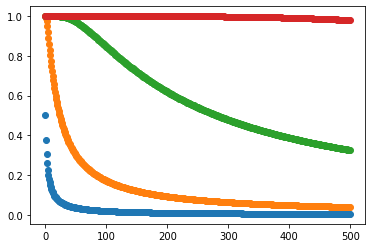
\includegraphics[width=0.56\textwidth]{figures/kvals.png}
\caption{Survival probability $S^{(k)}_n$ from \cref{m:eq:Snk} out to $500$
generations at exact criticality, $p=0.5$, for $k=1,10,100,1000$ (blue through to
red). A larger founding cohort buys longevity, but at criticality every curve is
still headed for zero.}
\label{m:fig:kvals}
\end{figure}

\begin{figure}[ht]
\centering
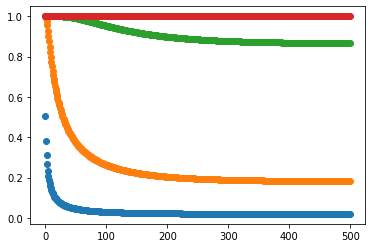
\includegraphics[width=0.45\textwidth]{figures/kvals505.png}
\hfill
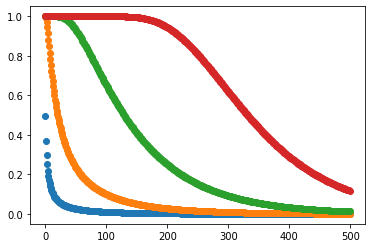
\includegraphics[width=0.45\textwidth]{figures/kvals495.png}
\caption{As \cref{m:fig:kvals}, but with $p$ displaced slightly from
criticality: $p=0.505$ on the left (supercritical), $p=0.495$ on the right
(subcritical). The benefit of a large initial cohort is acutely sensitive to
which side of $\tfrac12$ the process sits on. A displacement of half a per cent
separates curves that were nearly coincident in \cref{m:fig:kvals}.}
\label{m:fig:kvals2}
\end{figure}

\Cref{m:fig:kvals,m:fig:kvals2} show $S_n^{(k)}$ through $500$ generations for
$k=1,10,100,1000$. The effect visible in \cref{m:fig:kvals} --- that a larger
first cohort gives improved longevity --- is highly sensitive to criticality.
Persistence improves quickly as $p$ approaches $\tfrac12$ from below and
continues to improve dramatically into supercriticality, and the two panels of
\cref{m:fig:kvals2} differ only in the third decimal place of $p$.

\subsection*{Conditioning and apparent early growth}
\label{m:sec:earlyrep}

The conditioning of \cref{m:sec:condmean} has a mirror image which is worth
recording, because it shows that the effect is not confined to the subcritical
case.

Consider an ensemble of independent homogeneous birth--death processes, all with
the same constant rates, and retain only those that happen still to be alive at
some large time. The retained subpopulation is automatically enriched for early
rapid growth: a realisation that grew quickly at the outset is far more likely
to have escaped the early extinction risk documented in \cref{m:fig:earlySn},
and so far more likely to be in the retained set. No change in the underlying
rates is required to produce the enrichment, and the apparent slowdown that
follows is not a slowdown at all but a reversion to the mean. The effect is
known as the \emph{push of the past}, and was identified in a setting far from
the present one, as an explanation for a systematic pattern in longevity and
diversity data \cite{Budd2018}.

That is exactly the conditioning of \cref{m:sec:condmean} seen from the other
side. There a subcritical process was conditioned on survival and its mean
settled to $1/A(p)$ rather than decaying; here a critical or supercritical
process is conditioned on survival to a late time and its early growth appears
inflated. In both cases the conditioning, not the mechanism, does the work:
selection is being performed on paths after they have been generated.

The parallel suggests a modelling hypothesis that later chapters take up: that
early replication weighs heavily on eventual survival, even when later
per-capita rates are unchanged. \Cref{m:fig:earlySn} is the reason to take it
seriously, since the first few generations are where nearly all of the
extinction risk sits.

\FloatBarrier
